\documentclass[11pt,a4paper]{article}
\usepackage[T1]{fontenc}
\usepackage[utf8]{inputenc}
\usepackage{lmodern}
\usepackage{amsmath,amssymb,amsthm,mathtools,mathrsfs}
\usepackage{graphicx,float,xcolor,multicol}
\usepackage[shortlabels]{enumitem}
\usepackage[margin=27mm]{geometry}
\usepackage{microtype,needspace,placeins}
\usepackage{tikz,tikz-cd}
\usetikzlibrary{arrows.meta,calc,positioning,patterns,decorations.pathreplacing}
\usepackage[colorlinks=true,linkcolor=teal,urlcolor=teal,citecolor=teal]{hyperref}
\setlength{\parindent}{0pt}
\setlength{\parskip}{.6em}
\setcounter{secnumdepth}{0}
\allowdisplaybreaks
\raggedbottom
\providecommand{\cross}{\times}
\DeclareUnicodeCharacter{2020}{\ensuremath{\dagger}}
\DeclareMathOperator{\supp}{supp}
\DeclareMathOperator*{\esssup}{ess\,sup}
\providecommand{\chapter}{\section}
\newenvironment{tool}[2]{\subsection*{Tool #1 --- #2}}{}
\newcommand{\ToolRef}[1]{Tool #1}
\newcommand{\FigureTag}[2]{\textit{Figure #1}}
\newcommand{\Result}[1]{\subsection*{#1}}
\newcommand{\Application}[1]{\subsubsection*{Application\if\relax\detokenize{#1}\relax\else\space--- #1\fi}}
\newcommand{\ProofHeading}{\par\textit{Proof.}\space}
\newcommand{\ProofOf}[1]{\par\textit{Proof of #1.}\space}
\newcommand{\RemarkHeading}{\par\textbf{Remark.}\space}
\newcommand{\NoteHeading}{\par\textbf{Note.}\space}
\newcommand{\ExerciseHeading}{\par\textbf{Exercise.}\space}

% Rendering support only; mathematical text is in each independent post.
\usepackage{booktabs,array,longtable}
\definecolor{HandoutBlue}{HTML}{2F6690}
\definecolor{HandoutNavy}{HTML}{17365D}
\newtheorem{theorem}{Theorem}
\newtheorem{lemma}[theorem]{Lemma}
\newtheorem{proposition}[theorem]{Proposition}
\newtheorem{corollary}[theorem]{Corollary}
\newtheorem{conjecture}[theorem]{Conjecture}
\newtheorem{definition}{Definition}
\newtheorem{example}{Example}
\newtheorem{namedtoolcounter}{Tool}
\newenvironment{namedtool}[1]{\begin{namedtoolcounter}[#1]}{\end{namedtoolcounter}}
\newtheorem*{claim}{Claim}
\newtheorem*{remark}{Remark}
\newtheorem*{exercise}{Exercise}
\newtheorem*{question}{Question}
\newtheorem*{observation}{Observation}
\newcommand{\SourceChapter}[2]{\section*{#2}}
\newcommand{\Lecture}[2]{\section*{Lecture #1: #2}}
\newcommand{\unclear}[1]{\textit{[unclear: #1]}}
\newcommand{\sourcegap}{\textit{[unfinished in the source]}}
\DeclareMathOperator{\dist}{dist}
\DeclareMathOperator{\id}{id}
\DeclareMathOperator{\Hol}{Hol}
\DeclareMathOperator{\Per}{Per}
\DeclareMathOperator{\Fix}{Fix}
\DeclareMathOperator{\diam}{diam}
\DeclareMathOperator{\Var}{Var}
\DeclareMathOperator{\Leb}{Leb}
\DeclareMathOperator{\Hom}{Hom}
\DeclareMathOperator{\End}{End}
\DeclareMathOperator{\Ann}{Ann}
\DeclareMathOperator{\Spec}{Spec}
\DeclareMathOperator{\Max}{Max}
\DeclareMathOperator{\Ob}{Ob}
\DeclareMathOperator{\Tor}{Tor}
\DeclareMathOperator{\Ass}{Ass}
\DeclareMathOperator{\Mor}{Mor}
\DeclareMathOperator{\Fun}{Fun}
\DeclareMathOperator{\Nat}{Nat}
\DeclareMathOperator{\Cone}{Cone}
\DeclareMathOperator{\MCG}{MCG}
\DeclareMathOperator{\Aut}{Aut}
\DeclareMathOperator{\Deck}{Deck}
\DeclareMathOperator{\SL}{SL}
\DeclareMathOperator{\PSL}{PSL}
\DeclareMathOperator{\Area}{Area}
\DeclareMathOperator{\im}{im}
\DeclareMathOperator{\PSh}{PSh}
\newcommand{\CRing}{\mathsf{CRings}}
\newcommand{\AMod}{A\text{-}\mathsf{Mod}}
\newcommand{\Ab}{\mathsf{Ab}}
\newcommand{\Z}{\mathbb Z}
\newcommand{\Q}{\mathbb Q}
\newcommand{\R}{\mathbb R}
\newcommand{\C}{\mathbb C}
\newcommand{\N}{\mathbb N}
\newcommand{\kk}{\mathbb k}
\renewcommand{\aa}{\mathfrak a}
\newcommand{\bb}{\mathfrak b}
\newcommand{\pp}{\mathfrak p}
\newcommand{\qq}{\mathfrak q}
\newcommand{\mm}{\mathfrak m}
\newcommand{\nn}{\mathfrak n}
\newcommand{\rad}{\mathrm r}
\newcommand{\cat}[1]{\mathsf{#1}}
\setcounter{secnumdepth}{0}
\allowdisplaybreaks

\graphicspath{{figures/commutative-algebra/}}
\begin{document}
\section*{Sheaves, Stalks, and Ringed Spaces}
% BLOG-CONTENT-BEGIN
\subsection{Sheaves}
\setcounter{definition}{17}\begin{definition}
Let $X$ be a topological space. A \emph{presheaf} $\mathcal F$ consists of:
\begin{enumerate}[label=(\roman*)]
\setcounter{enumi}{0}\item An abelian group $\mathcal F(U)$ for every open $U\subseteq X$.
\setcounter{enumi}{1}\item For open $V\subseteq U$, a group morphism $\rho_{UV}:\mathcal F(U)\to\mathcal F(V)$ such that $\rho_{UU}=\id_{\mathcal F(U)}$ and, for open $W\subseteq V\subseteq U$, $\rho_{VW}\circ\rho_{UV}=\rho_{UW}$.
\end{enumerate}
\end{definition}
\setcounter{definition}{18}\begin{definition}
A presheaf $\mathcal F$ is a \emph{sheaf} if, for $U=\bigcup_i U_i$, the sequence
\[
0\longrightarrow\mathcal F(U)\xrightarrow{d_0}\prod_i\mathcal F(U_i)
\xrightarrow{d_1}\prod_{i,j}\mathcal F(U_i\cap U_j)
\]
is exact, where $d_0:s\mapsto s|_{U_i}$ and
% Source page 5
$d_1:\prod_i s_i\mapsto s_i|_{U_i\cap U_j}-s_j|_{U_i\cap U_j}$.
The condition $\ker d_0=0$ encodes uniqueness, and $\operatorname{im}d_0=\ker d_1$ encodes gluing.
\end{definition}
\setcounter{definition}{19}\begin{definition}
The \emph{stalk} of $\mathcal F$ at $p$, denoted $\mathcal F_p$, is
\[\{(f,U)\mid p\in U,\ f\in\mathcal F(U)\}/{\sim},\]
where $(f,U)\sim(g,V)$ if there exists $W\subset U,V$, $p\in W$, with $\rho_{UW}f=\rho_{VW}g$. These are \emph{germs at $p$}.
% The source repeats f on the right-hand side; corrected to the already named g.
\end{definition}
\begin{remark}
One can also set $\mathcal F_p:=\operatorname{colim}_{p\in U}\mathcal F(U)$.
\end{remark}
\setcounter{definition}{20}\begin{definition}
A nonempty poset $(S,\ge)$ is \emph{filtered} if, for every $x,y\in S$, there exists $z$ such that $x,y\ge z$. More generally, a category $C$ is filtered if it is nonempty and:
\begin{enumerate}[label=(\roman*)]
\setcounter{enumi}{0}\item For $x,y\in C$, there exists $z$ with arrows $x\to z$ and $y\to z$.
\setcounter{enumi}{1}\item For every $u,v:x\to y$, there exists $w:y\to z$ such that $w\circ u=w\circ v$.
\end{enumerate}
\begin{figure}[H]\centering
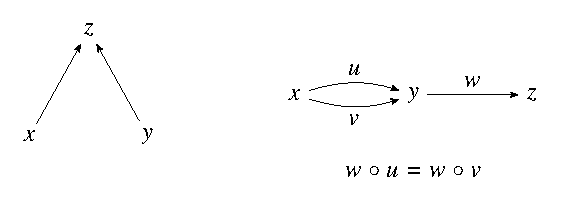
\includegraphics[width=.66\textwidth]{ca6-fig-02.pdf}
\end{figure}
\end{definition}
Suppose $\mathcal I$ is a filtered indexing category. Any diagram indexed by $\mathcal I$ has the following colimit:
% Source page 6
\[
\varinjlim_{i\in\mathcal I}A_i
=\left\{(a_i,i)\in\coprod_{i\in\mathcal I}A_i\right\}/{\sim},
\]
where $(a_i,i)\sim(a_j,j)$ if there exist $f:A_i\to A_k$ and $g:A_j\to A_k$ with $f(a_i)=g(a_j)$. Thus \mbox{$\mathcal F_p=\varinjlim_{p\in U}\mathcal F(U)$}.
% The source repeats f(a_j); corrected to g(a_j), matching the displayed domains.
For a sheaf $\mathcal F$, one has $\mathcal F(U)\to\mathcal F_p$, $s\mapsto s_p$, for $p\in U$.
\setcounter{theorem}{31}\begin{lemma}
If $s,t\in\mathcal F(X)$ and $s_x=t_x$ for every $x\in X$, then $s=t$.
\end{lemma}
\begin{proof}
Without loss of generality, assume $t=0$. For every $x\in X$, there exists $U_x$ such that $s|_{U_x}=0$. Hence $s\equiv0$ by the uniqueness axiom of $\mathcal F$.
\end{proof}
\paragraph{Morphisms of (pre)sheaves.}
A morphism $\alpha:\mathcal F\to\mathcal G$ is a collection of group morphisms $\alpha(U):\mathcal F(U)\to\mathcal G(U)$ for every open $U\subseteq X$, compatible with all restriction maps.
\paragraph{Sheafification.}
Given a presheaf $\mathcal F$, there exists a sheaf $\mathcal F^+$, unique up to unique isomorphism, with $\theta:\mathcal F\to\mathcal F^+$ such that, for every morphism $\alpha:\mathcal F\to\mathcal G$ with $\mathcal G$ a sheaf, there is a unique $\widetilde\alpha$ making the diagram commute.
\begin{figure}[H]\centering
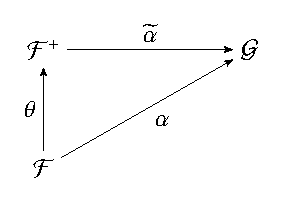
\includegraphics[width=.48\textwidth]{ca6-fig-03.pdf}
\end{figure}
\[
\mathcal F^+(U):=\left\{
f:U\to\coprod_{x\in U}\mathcal F_x\ \middle|\
\begin{array}{l}
f(x)\in\mathcal F_x\text{ for every }x\in U;\\
\text{for every }x\in U\text{ there exist an open }V\ni x\text{ and }s\in\mathcal F(V)\\
\text{such that }f(y)=s_y\text{ for every }y\in V
\end{array}\right\}.
\]
% Source page 7
\subsection{Ringed topological spaces}
\setcounter{definition}{21}\begin{definition}[Ringed and locally ringed spaces]
\begin{enumerate}[label=(\roman*)]
\setcounter{enumi}{0}\item $(X,\mathcal O_X)$ is a \emph{ringed topological space} if $X\in\mathsf{Top}$ and $\mathcal O_X$ is a sheaf of rings. It is a \emph{locally ringed space} if $\mathcal O_{X,x}$ is a local ring for every $x\in X$. Here $\mathcal O_X$ is the \emph{structure sheaf}, and $\mathcal O_{X,x}/\mm_x$ is the \emph{residue field}.
\setcounter{enumi}{1}\item A morphism $(f,f^{\#}):(X,\mathcal O_X)\to(Y,\mathcal O_Y)$ of locally ringed spaces consists of a continuous map $f:X\to Y$ and a sheaf map $f^{\#}:\mathcal O_Y\to f_*\mathcal O_X$, where $f_*\mathcal F(V):=\mathcal F(f^{-1}(V))$, such that
\[
f_x^{\#}:\mathcal O_{Y,f(x)}\longrightarrow \mathcal O_{X,x}
\]
is a local homomorphism, that is, $f_x^{\#}(\mm_{f(x)})\subseteq\mm_x$.
\setcounter{enumi}{2}\item $(f,f^{\#})$ is an \emph{open immersion} if $f$ is an open embedding and $f_x^{\#}$ is an isomorphism for every $x\in X$. It is a \emph{closed immersion} if $f$ is a closed embedding and $\mathcal O_Y\to f_*\mathcal O_X$ is surjective.
\end{enumerate}
\end{definition}
For $X=\Spec(A)$, define $\mathcal O_X(D(f)):=A_f$. On the left, $D(f)$ is the locus where $f$ does not vanish; on the right, $A_f$ is the ring in which $f$ is invertible.
\setcounter{theorem}{32}\begin{lemma}
$V(I)\subseteq V(J)$ if and only if $J\subseteq\sqrt I$.
\end{lemma}
Also, $D(g)\subseteq D(f)$ implies $g\in\sqrt{(f)}$, so there exist $m\ge1$ and $b\in A$ with $g^m=fb$.
% Source page 8
Thus $f$ is invertible in $A_g$, giving a map $A_f\to A_g$. These restriction maps define a sheaf on the basis of distinguished open sets and extend uniquely to the structure sheaf $\mathcal O_X$. Note that $\mathcal O_X(X)=A$, and for every $\pp\in X$, $\mathcal O_{X,\pp}:=A_{\pp}$ is local. Therefore $(X,\mathcal O_X)$ is a locally ringed topological space.
\setcounter{definition}{22}\begin{definition}
\begin{enumerate}[label=(\roman*)]
\setcounter{enumi}{0}\item An \emph{affine scheme} is a locally ringed topological space isomorphic to some $(X,\mathcal O_X)$ as above.
\end{enumerate}
\end{definition}
% BLOG-CONTENT-END
\end{document}
